\section{Criteria to determine candidate elements to inhibit Mg corrosion}
\label{chap:Mg_H:sec:criteria}

The following three criteria were applied to determine if an alloying element could potentially inhibit Mg corrosion by slowing down the \ac{HER} as the cathodic reaction on surfaces of Fe-rich second-phase particles. (1) The alloying element must show a thermodynamic preference for bulk Fe over bulk Mg. (2) The alloying element must be thermodynamically more stable on Fe surfaces than in bulk Fe. (3) The adsorption energies of a lone H atom on Fe surfaces with an alloying element in their topmost layers should be significantly reduced (or enhanced) relative to the adsorption energies of a lone H atom on pure Fe surfaces, suggesting possible interference with $\text{H}_2$(g) formation and a consequent decrease in the \ac{HER} rate. Therefore, criterion 3 requires that a potential candidate significantly increase or reduce H adsorption strength on Fe particle surfaces. 


The second and third criteria require the investigation of specific Fe surfaces. The Wulff plot shows (100) and (110) surfaces of a \ac{BCC} Fe single crystal are the two-major low-index surfaces at equilibrium conditions; (100) and (110) occupy more than $\text{50}\%$ of the \ac{BCC} Fe surface area and have the lowest energies \cite{tran2016surface}. Other high-index surfaces are also combinations of these two surfaces with steps. Therefore, our high-throughput search was conducted on models constructed with either (100) or (110) surfaces of \ac{BCC} Fe.  

\begingroup
\begin{figure}[!ht]
  \centering
  \subfigure{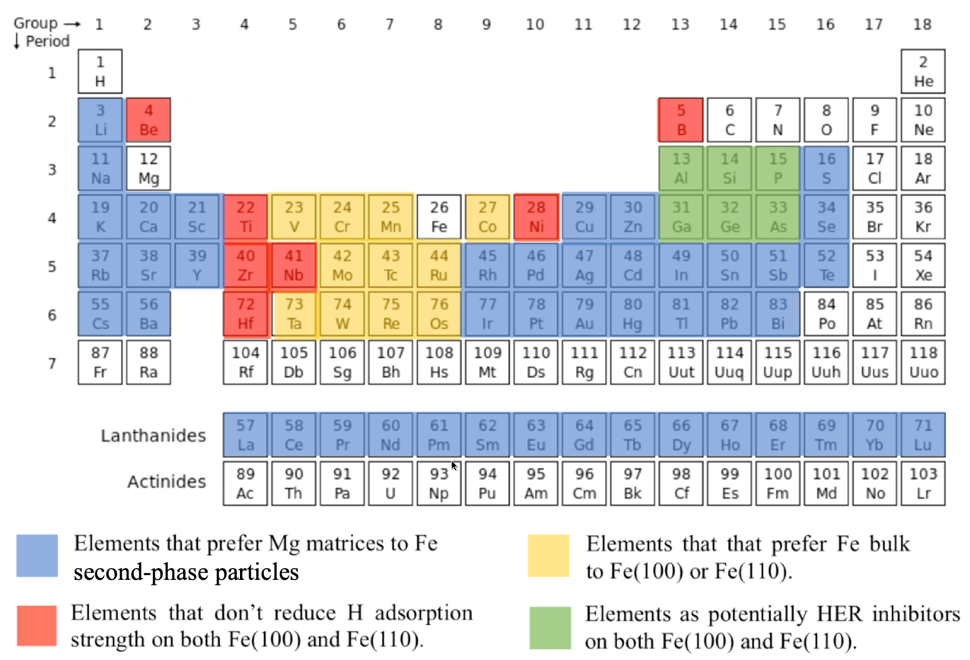
\includegraphics[width=1.0\linewidth]{Chap3/plots/Fig4.png}}
  \caption[Summary of the high-throughput search for alloying elements that can inhibit HER on surfaces of Fe second-phase particles in Mg matrix]{Summary of the high-throughput search for alloying elements that can inhibit \ac{HER} on surfaces of Fe second-phase particles in Mg matrix. All investigated alloying elements are labeled in colors (blue, yellow, red and green). Different colors describe the search results for the corresponding alloying elements as explained in the figure legends. (White periodic table from Wikimedia Commons)}
  \label{Chap:Mg_H:fig4}
\end{figure}
\endgroup

% \section{First-principles calculation methods and high-throughput search approach}
% \label{chap:Mg_H:sec:calculation}

The first criterion requires that a Mg corrosion-inhibiting element must have a thermodynamic preference for bulk Fe over bulk Mg. Hence, models aimed at examining bulk segregation energetics were constructed. To simulate bulk Fe, we constructed a 4x4x4(64 atoms) supercell (each primitive cell consists of 1 Fe atom). To simulate bulk Mg, we constructed a 4x4x2 supercell (64 atoms) with each primitive cell consisting of 2 Mg atoms. An element (e.g. As) was then placed at an Fe substitutional site in the bulk Fe supercell and at a Mg substitutional site in the Mg bulk supercell, as shown in Figs. 2(a) and 2(b), respectively.


To address the second criterion (an element must have a thermodynamic preference for Fe (100) and Fe (110) surfaces rather than for bulk Fe), four models aimed at examining Fe surface segregation energetics were constructed. Each consisted of 40 atoms in the Fe (100) and Fe (110) slabs with 10 layers of 2x2 surface periodicity and a 12$\angstrom$ vacuum.  Two of the models contained an element placed at an Fe substitutional site in the top surface layers of Fe (100) and Fe (110) (i.e. where the \ac{HER} is expected to occur). These models are shown in Figs. 2(c) and 2(d), respectively. For the remaining two models, also shown in Figs. 2(c) and 2(d), an element (e.g. As) was placed at an Fe substitutional site five layers below the top surface.

\newpage
\begingroup
\begin{figure}[!ht]
  \centering
  \subfigure[]{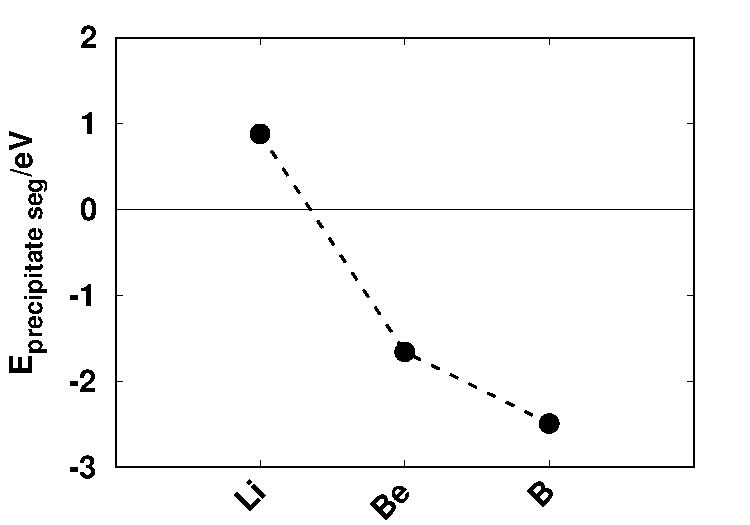
\includegraphics[width=0.46\linewidth]{Chap3/plots/Fig5a.pdf}}\label{Chap:Mg_H:fig:5a}
  \subfigure[]{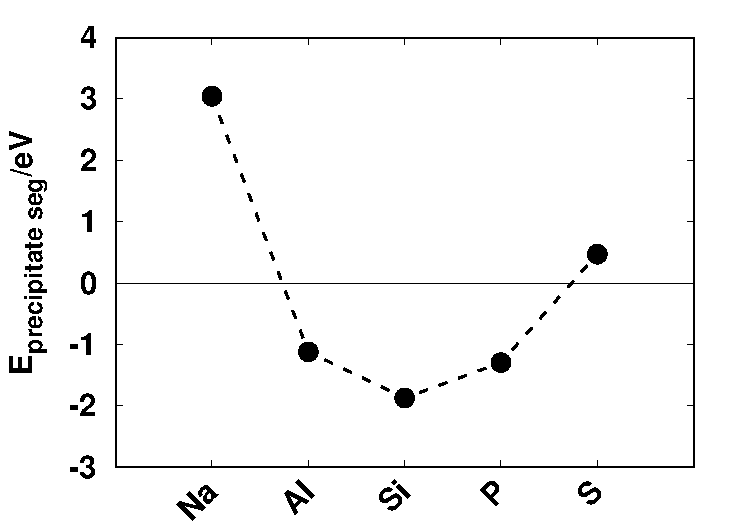
\includegraphics[width=0.46\linewidth]{Chap3/plots/Fig5b.pdf}}\label{Chap:Mg_H:fig:5b}
  \\
  \subfigure[]{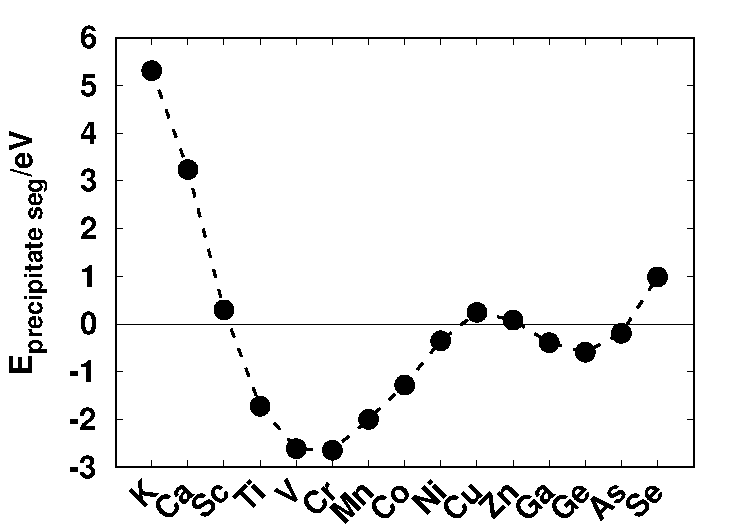
\includegraphics[width=0.46\linewidth]{Chap3/plots/Fig5c.pdf}}\label{Chap:Mg_H:fig:5c}
  \subfigure[]{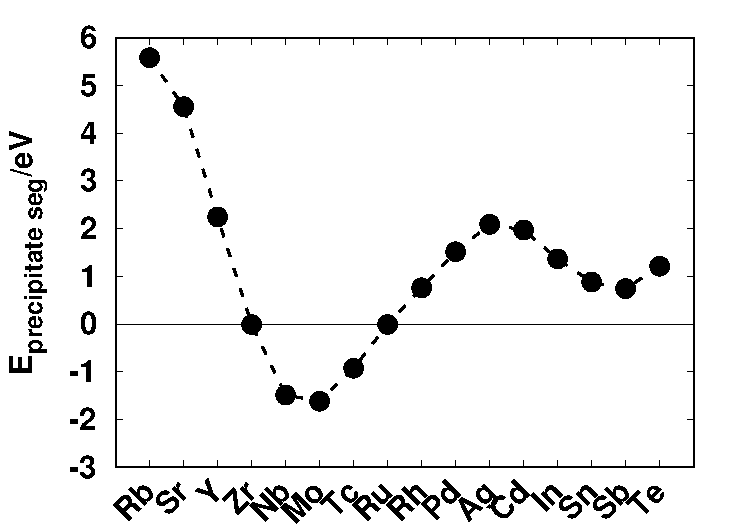
\includegraphics[width=0.46\linewidth]{Chap3/plots/Fig5d.pdf}}\label{Chap:Mg_H:fig:5d}
  \\
  \subfigure[]{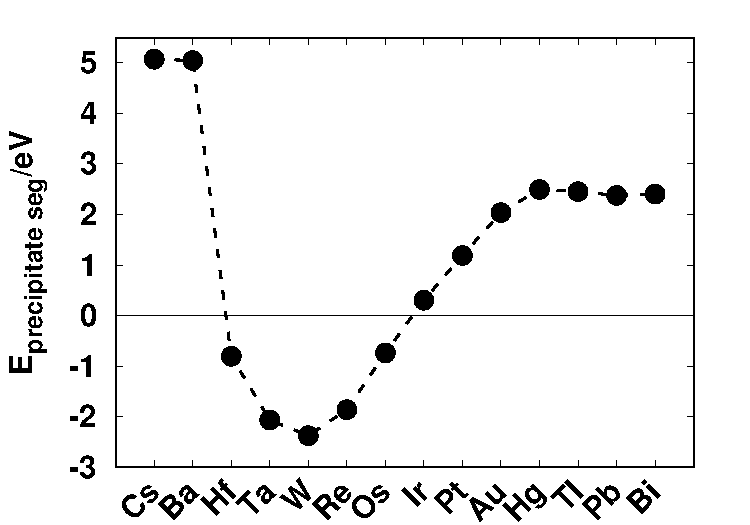
\includegraphics[width=0.46\linewidth]{Chap3/plots/Fig5e.pdf}}\label{Chap:Mg_H:fig:5e}
  \subfigure[]{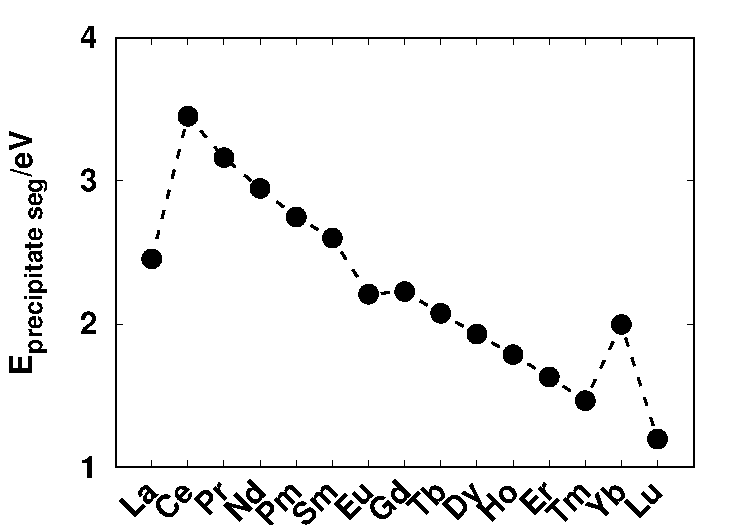
\includegraphics[width=0.46\linewidth]{Chap3/plots/Fig5f.pdf}}\label{Chap:Mg_H:fig:5f}
\caption[Segregation energies to bulk second-phase particles]{Segregation energies to bulk second-phase particles $E_{particle seg}$ defined in Eq. \ref{Chap:Mg_H:eq:particle_seg} for the 68 potential alloying elements. Preference for a \ac{BCC} Fe particle over the bulk \ac{HCP} Mg requires that an alloying element should have a significantly negative value of $E_{particle seg}$. (a)~(e): Elements in Row 2, 3, 4, 5 and 6 of the periodic table, respectively. (f) Lanthanide Elements. Elements with negative Eparticle seg are narrowed to 24: Be, B, Al, Si, P, Ti, V, Cr, Mn, Co, Ni, Ga, Ge, As, Zr, Nb, Mo, Tc, Ru, Hf, Ta, W, Re and Os.}
  \label{Chap:Mg_H:fig5}
\end{figure}
\endgroup

To address the third criterion that pertains to affecting H adsorption energies and possibly the HER rate, H adsorption energetics were investigated with both a single H atom adsorbed ($\frac{1}{4}$ \ac{ML}) at different sites on Fe (100) and Fe (110) with (2x2) in-plane periodicity and an alloying element substituting an Fe atom in the top surface layer. On a (2x2) Fe (100) with a substitutional alloying atom in the top layer, there are four possible H adsorption sites as shown in Fig. \ref{Chap:Mg_H:fig:3a}: (1) a top site directly above 1 Fe atom or 1 alloying atom substituting for an Fe surface atom, (2) a bridge site I with 1 Fe atom and 1 alloying atom nearest neighbors (NNs), (3) a bridge site II with 2 Fe atoms as NNs, (4) a hollow site with 3 Fe atoms and 1 alloying atom NNs. On a (2x2) Fe (110) with a substitutional alloying atom in the top layer, there are five H adsorption sites of interest as shown in Fig. \ref{Chap:Mg_H:fig:3b}: (1) a top site directly above 1 Fe atom or 1 alloying atom, (2) a bridge site I with 1 Fe atom and 1 alloying atom as NNs, (3) a bridge site II with 2 Fe atoms as NNs, (4) a hollow site I with 2 Fe atoms and 1 alloying atom as NNs, (5) a hollow site II with 3 Fe atoms as NNs.


The computational engine that provided the energetics used to evaluate the three criteria for each of the 68 candidate alloying elements was the implementation of \ac{DFT} in the \ac{VASP}. Each model was spin-polarized to account for \ac{BCC} Fe ferromagnetism. All-electron \ac{PAW} potentials were employed for the elemental constituents with the \ac{GGA} of \ac{PBE} for the exchange-correlation energy functional, $\mu_{xc}$, and the interpolation formula of Vosko et al. \cite{vosko1980accurate}. Using a plane wave cutoff energy of at 450.0 eV, the total energy for all models was converged to $10^{−7}$ eV/cell, and the force components on each atom were relaxed to less than $10^{−3}$ eV/Å. The reciprocal space of Fe (110), Fe (100) and bulk supercells were sampled with (16x16x1), (14x14x1), and (8x8x8) k-point grids, respectively. Each grid was generated using the Monkhorst-Pack scheme \cite{monkhorst1976special}. A 20$\angstrom$x20$\angstrom$x20$\angstrom$ supercell with a $\text{H}_2$ molecule in the middle was used for this calculation. The reciprocal space was sampled with a (1x1x1) Gamma centered k-points grid. Using a plane wave cutoff energy of at 450.0 eV, the total energy for all models was converged to $10^{−7}$ eV/cell.


Two successive structural optimizations (adapting basis vectors and computational grids to the cell parameters) were conducted on the bulk solids to ensure that the cell energies and structural parameters were fully converged. A \ac{VASP}-optimized lattice parameter of 2.83 $\angstrom$ for \ac{BCC} Fe was computed (the experimental room temperature value is 2.87 $\angstrom$ \cite{kohlhaas1967temperature}) along with a 2.197 $\mu B/atom$ spin moment. Our computed spin moment is in good agreement with the 2.2 $\mu B/atom$ value from the \ac{DFT} study of Tiago et al. \cite{tiago2006evolution}. For \ac{HCP} Mg, the VASP-optimized lattice parameters are: a=3.19 $\angstrom$, c/a = 1.62 (the room temperature experimental values are: a=3.32 $\angstrom$, c/a = 1.62 \cite{wrobel2012thermodynamic}). DFT calculations predict Fe (110) to have the lowest surface energy (2.40 $J/m^2$) and Fe (100) to have the second lowest surface energy (2.45 $J/m^2$), in accord with previous DFT studies of Fe surfaces \cite{hung2002first}.  Experiments, however, identify (100) as having the lowest surface energy \cite{tyson1977surface}. Possible reasons for the disparity between DFT and experiments are provided by Hung et al. \cite{hung2002first}.

\newpage
\begingroup
\begin{figure}[!ht]
  \centering
  \subfigure[]{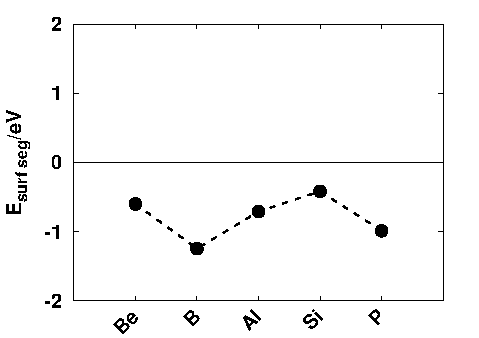
\includegraphics[width=0.49\linewidth]{Chap3/plots/Fig6a.pdf}}\label{Chap:Mg_H:fig:6a}
  \subfigure[]{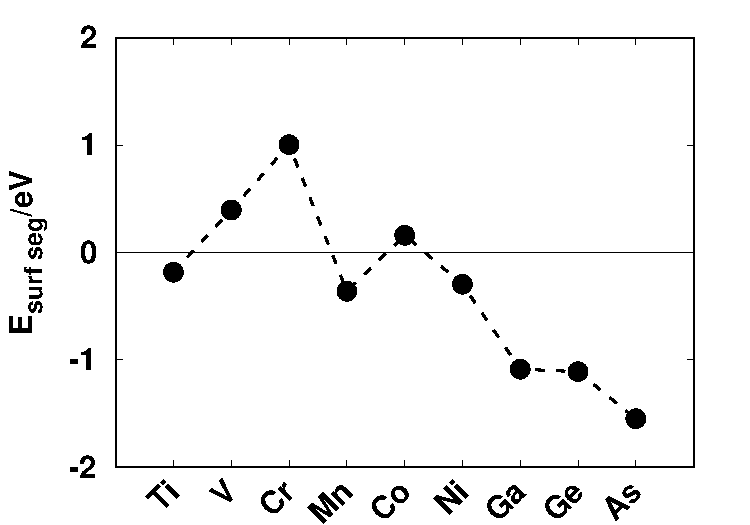
\includegraphics[width=0.49\linewidth]{Chap3/plots/Fig6b.pdf}}\label{Chap:Mg_H:fig:6b}
  \\
  \subfigure[]{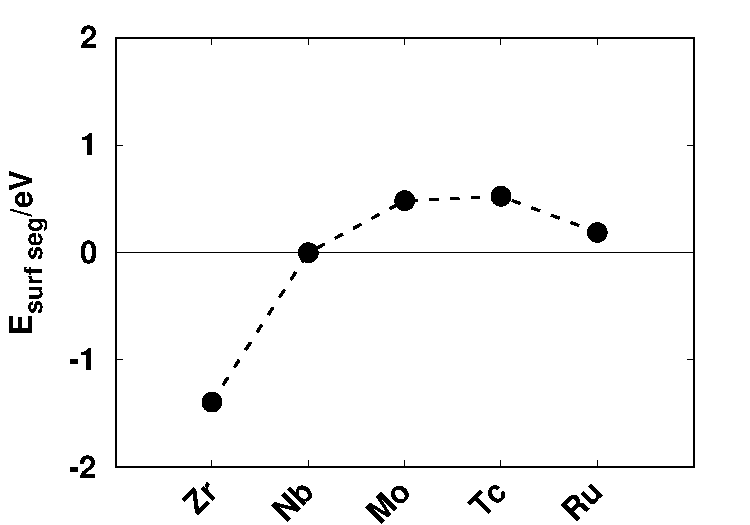
\includegraphics[width=0.49\linewidth]{Chap3/plots/Fig6c.pdf}}\label{Chap:Mg_H:fig:6c}
  \subfigure[]{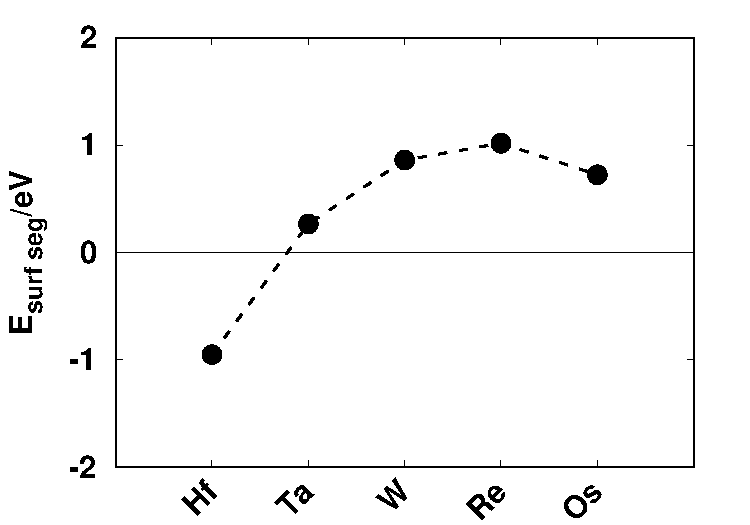
\includegraphics[width=0.49\linewidth]{Chap3/plots/Fig6d.pdf}}\label{Chap:Mg_H:fig:6d}
\caption[Surface segregation energies for Fe (100) of 24 alloying elements]{Segregation energies $E_{surf seg}$ defined in Eq. \ref{Chap:Mg_H:eq:surf_seg} for Fe (100) of 24 alloying elements narrowed from the first screening round. A qualified alloy candidate should have a strongly negative value of $E_{surf seg}$. (a): Elements in Row 2 and 3 of the periodic table. (b)~(d): Elements in Row of 4, 5 and 6 of the periodic table, respectively.}
  \label{Chap:Mg_H:fig6}
\end{figure}
\endgroup

Other than H adsorption energetics, there are two other criteria that are important as mentioned in Section 2.1: (1) an alloying element X should be more thermodynamically stable in bulk \ac{BCC} Fe instead of bulk \ac{HCP} Mg, (2) an alloying element X should segregate to an Fe surface rather than remaining in bulk Fe. Regarding the first criterion, we calculated the segregation energy to the second-phase particle, $E_{particle seg}$, via
\begin{align}
 E_{particle seg} = (\frac{63}{64}E_{Mg64} + E_{Fe63}X) - (E_{Mg63}X + \frac{63}{64}E_{Fe64})
 \label{Chap:Mg_H:eq:particle_seg}
\end{align}
where $E_{Mg64}$, $E_{Fe63X}$, $E_{Mg63X}$, and $E_{Fe64}$ are the total energies of 64-atom supercells for pure bulk HCP Mg, bulk \ac{BCC} Fe with 1 substitutional X atom (see Fig. \ref{Chap:Mg_H:fig:2a}), bulk HCP Mg with 1 substitutional X atom (see Fig. \ref{Chap:Mg_H:fig:2b}), and pure bulk \ac{BCC} Fe, respectively. A negative value of $E_{particle seg}$ for a given X means that it is energetically favorable for X to bind to bulk Fe instead of segregating to bulk Mg. The results show that a substitutional As atom has an energetic preference for bulk Fe over bulk Mg using the models shown in Fig. \ref{Chap:Mg_H:fig:2a} and \ref{Chap:Mg_H:fig:2b}, with a computed segregation energy of -0.19 eV.

\newpage
\begingroup
\begin{figure}[!ht]
  \centering
  \subfigure[]{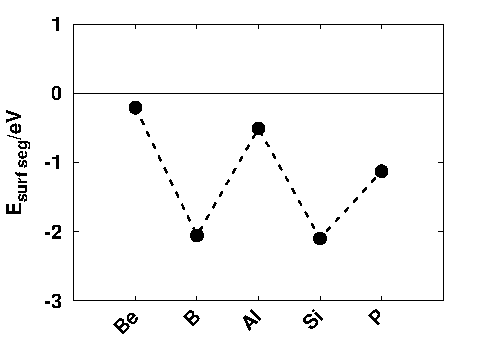
\includegraphics[width=0.49\linewidth]{Chap3/plots/Fig7a.pdf}}\label{Chap:Mg_H:fig:7a}
  \subfigure[]{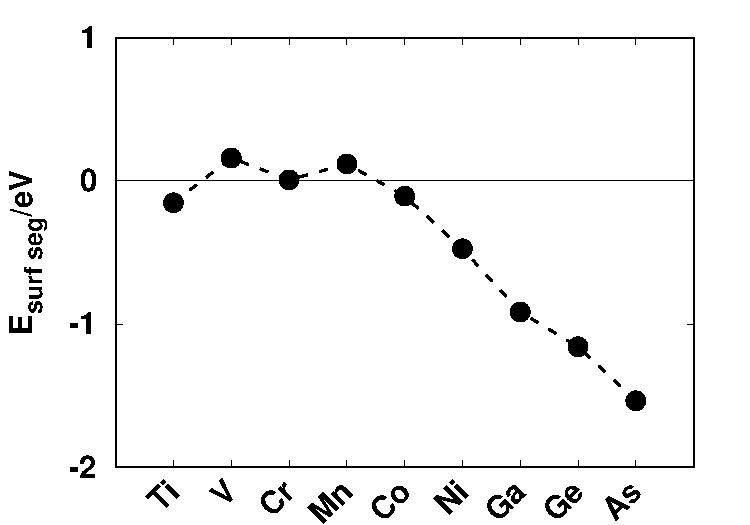
\includegraphics[width=0.49\linewidth]{Chap3/plots/Fig7b.pdf}}\label{Chap:Mg_H:fig:7b}
  \\
  \subfigure[]{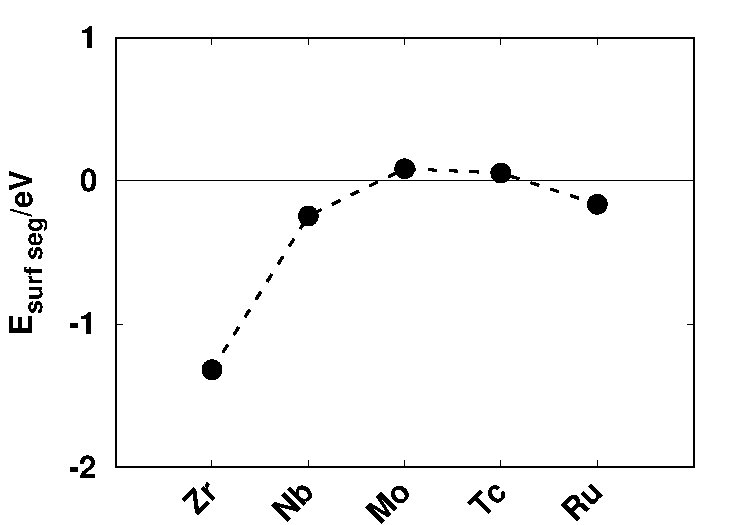
\includegraphics[width=0.49\linewidth]{Chap3/plots/Fig7c.pdf}}\label{Chap:Mg_H:fig:7c}
  \subfigure[]{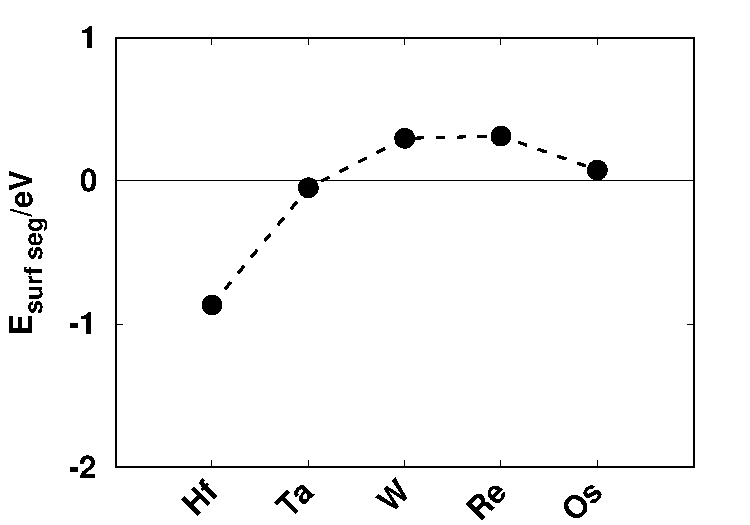
\includegraphics[width=0.49\linewidth]{Chap3/plots/Fig7d.pdf}}\label{Chap:Mg_H:fig:7d}
\caption[Surface segregation energies for Fe (110) of 24 alloying elements]{Segregation energies $E_{surf seg}$ defined in Eq. \ref{Chap:Mg_H:eq:surf_seg} for Fe (110) of 24 alloying elements narrowed from the first screening round. A qualified alloy candidate should have a strongly negative value of $E_{surf seg}$. (a): Elements in Row 2 and 3 of the periodic table. (b)~(d): Elements in Row of 4, 5 and 6 of the periodic table, respectively.}
  \label{Chap:Mg_H:fig7}
\end{figure}
\endgroup

Regarding the second criterion, we calculated the surface segregation energy of a substitutional alloying atom, $E_{surf seg}$, via:
\begin{align}
 E_{surf seg} = E_{surf} - E_{bulk}
 \label{Chap:Mg_H:eq:surf_seg}
\end{align}
where $E_{surf}$ and $E_{bulk}$ are the \ac{DFT}-computed energies of the corresponding surface slab with a substitutional alloying atom in the top surface layer (left figure in either Fig. \ref{Chap:Mg_H:fig:2c} or \ref{Chap:Mg_H:fig:2d}) and the surface slab with a substitutional alloying atom inside the bulk (right figure in either Fig. \ref{Chap:Mg_H:fig:2c} or \ref{Chap:Mg_H:fig:2d}), respectively). A negative $E_{surf seg}$ suggests that an alloying element will preferentially occupy an Fe site in the top surface layer instead of a site within bulk Fe. The results show that As prefers Fe (100) and Fe (110) instead of bulk Fe with computed segregation energies of -1.55 eV and -1.54 eV, respectively. Similar computations based on Eq. \ref{Chap:Mg_H:eq:particle_seg} and \ref{Chap:Mg_H:eq:surf_seg} were conducted for the other 67 elements noted in Fig. \ref{Chap:Mg_H:fig4} and detailed below.

The H adsorption energy, $E_{ad}^H$, was computed from  
\begin{align}
 E_{ad}^{H} = E_{H/slab} - E_{slab} - \frac{1}{2}E_{H_2}(g)
 \label{Chap:Mg_H:eq:H_ads}
\end{align}

where $E_{H/slab}$ and $E_{slab}$ are the total energies of supercells of an Fe surface slab with/without adsorbed H atoms, respectively. $\text{H}_2$(g) is the energy of an isolated hydrogen gas molecule. Thus, the hydrogen adsorption strength is stronger with a more negative value of $E_{ad}^H$. The most stable H adsorption site on pure Fe (100) is the hollow site noted in Fig. \ref{Chap:Mg_H:fig:3a} with $E_{ad}^H$ = -0.38 eV. With an As atom substituting an Fe atom in the top surface layer of Fe (100), Table \ref{Chap:Mg_H:tab:H_ads} shows that $E_{ad}^H$ at the hollow site with an As NN in Fig. \ref{Chap:Mg_H:fig:3a} changes to -0.22 eV/atom. If H is initially placed at the top site above the substitutional As atom in the top layer of Fe (100), an unfavorable $E_{ad}^H$ = 0.67 eV is substantially different than the $E_{ad}^H$ = 0.20 eV for H at the top site of pure Fe (100) as listed in Table \ref{Chap:Mg_H:tab:H_ads}. If H is initially placed at bridge site I in Fig. \ref{Chap:Mg_H:fig:3a}, it moves to the top site above the Fe NN during \ac{VASP} optimization. $E_{ad}^H$ at the bridge site II in Fig. \ref{Chap:Mg_H:fig:3a} is very similar to $E_{ad}^H$ at the bridge site of pure Fe (100) because there is no As as the NN.

\newpage
\begingroup
\begin{figure}[!ht]
  \centering
  \subfigure[]{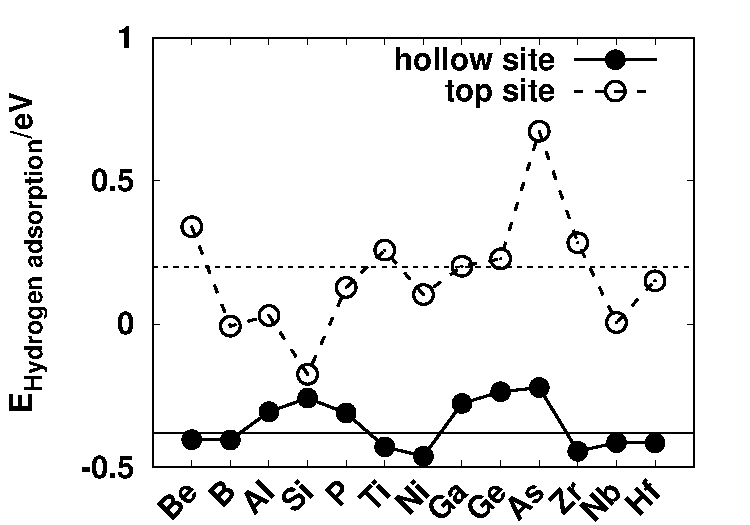
\includegraphics[width=0.6\linewidth]{Chap3/plots/Fig8a.pdf}}\label{Chap:Mg_H:fig:8a}
  \subfigure[]{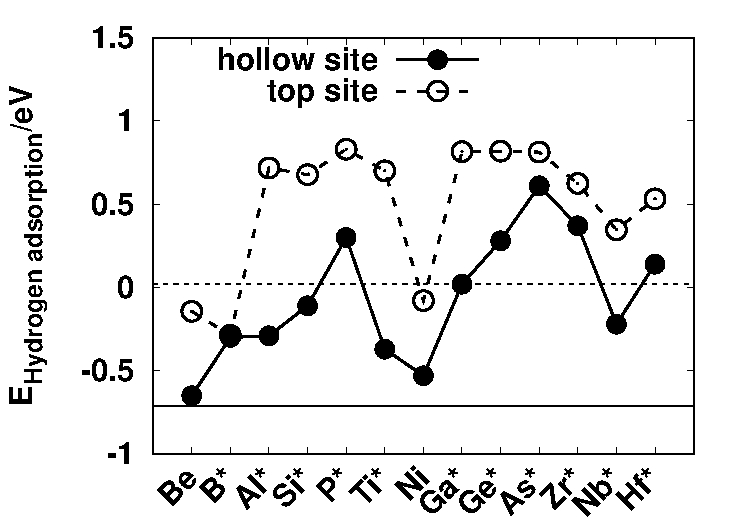
\includegraphics[width=0.6\linewidth]{Chap3/plots/Fig8b.pdf}}\label{Chap:Mg_H:fig:8b}
\caption[H adsorption energies on Fe (100) and Fe (110) with the 13 alloying elements that pass the second screening round]{H adsorption energies $E_{ad}^H$ defined in Eq. \ref{Chap:Mg_H:eq:H_ads} on Fe (100) and Fe (110) with the 13 alloying elements that pass the second screening round.  (a) H adsorption energies at the hollow site and the top site on Fe (100) with different alloying elements. Their surface geometry is shown in Fig. \ref{Chap:Mg_H:fig:3a}. The horizontal solid and dash lines are the hydrogen adsorption energy at hollow site and top site of pure Fe (100), respectively. (b) H adsorption energies at the hollow site I and the top site on Fe (110) with different alloying elements. Their surface geometry is shown in Fig. \ref{Chap:Mg_H:fig:3b}. The horizontal solid and dash lines are the hydrogen adsorption energy at hollow site I and top site on a pure Fe surface, respectively. H adsorption energies at the hollow site I on Fe (110) surfaces with B, Al, Si, P, Ti, Ga, Ge, As, Zr, Nb and Hf (marked with *) were computed by only allowing H and surface atoms to relax in the direction normal to the Fe (110).}
  \label{Chap:Mg_H:fig8}
\end{figure}
\endgroup